\subsection{Beispiel einer konkreten Klassifikation}
    Dieses Kapitel stellt ein Beispiel für eine konkrete Klassifikation vor,
    die nach dem oben beschriebenen Modell in der Datenbank gespeichert wird.
    % TODO: Erwähnen, dass hier eine Seite der KSW genutzt wird?
    Abbildung \ref{image:dbDataModelExampleOverviewPart1} zeigt den ersten Teil dieses Beispiels.
    Hier wird zunächst auf die ausführliche Startellung der Eigenschaften der Beziehungen verzichtet.

    \begin{figure}[htb]
        \centering
        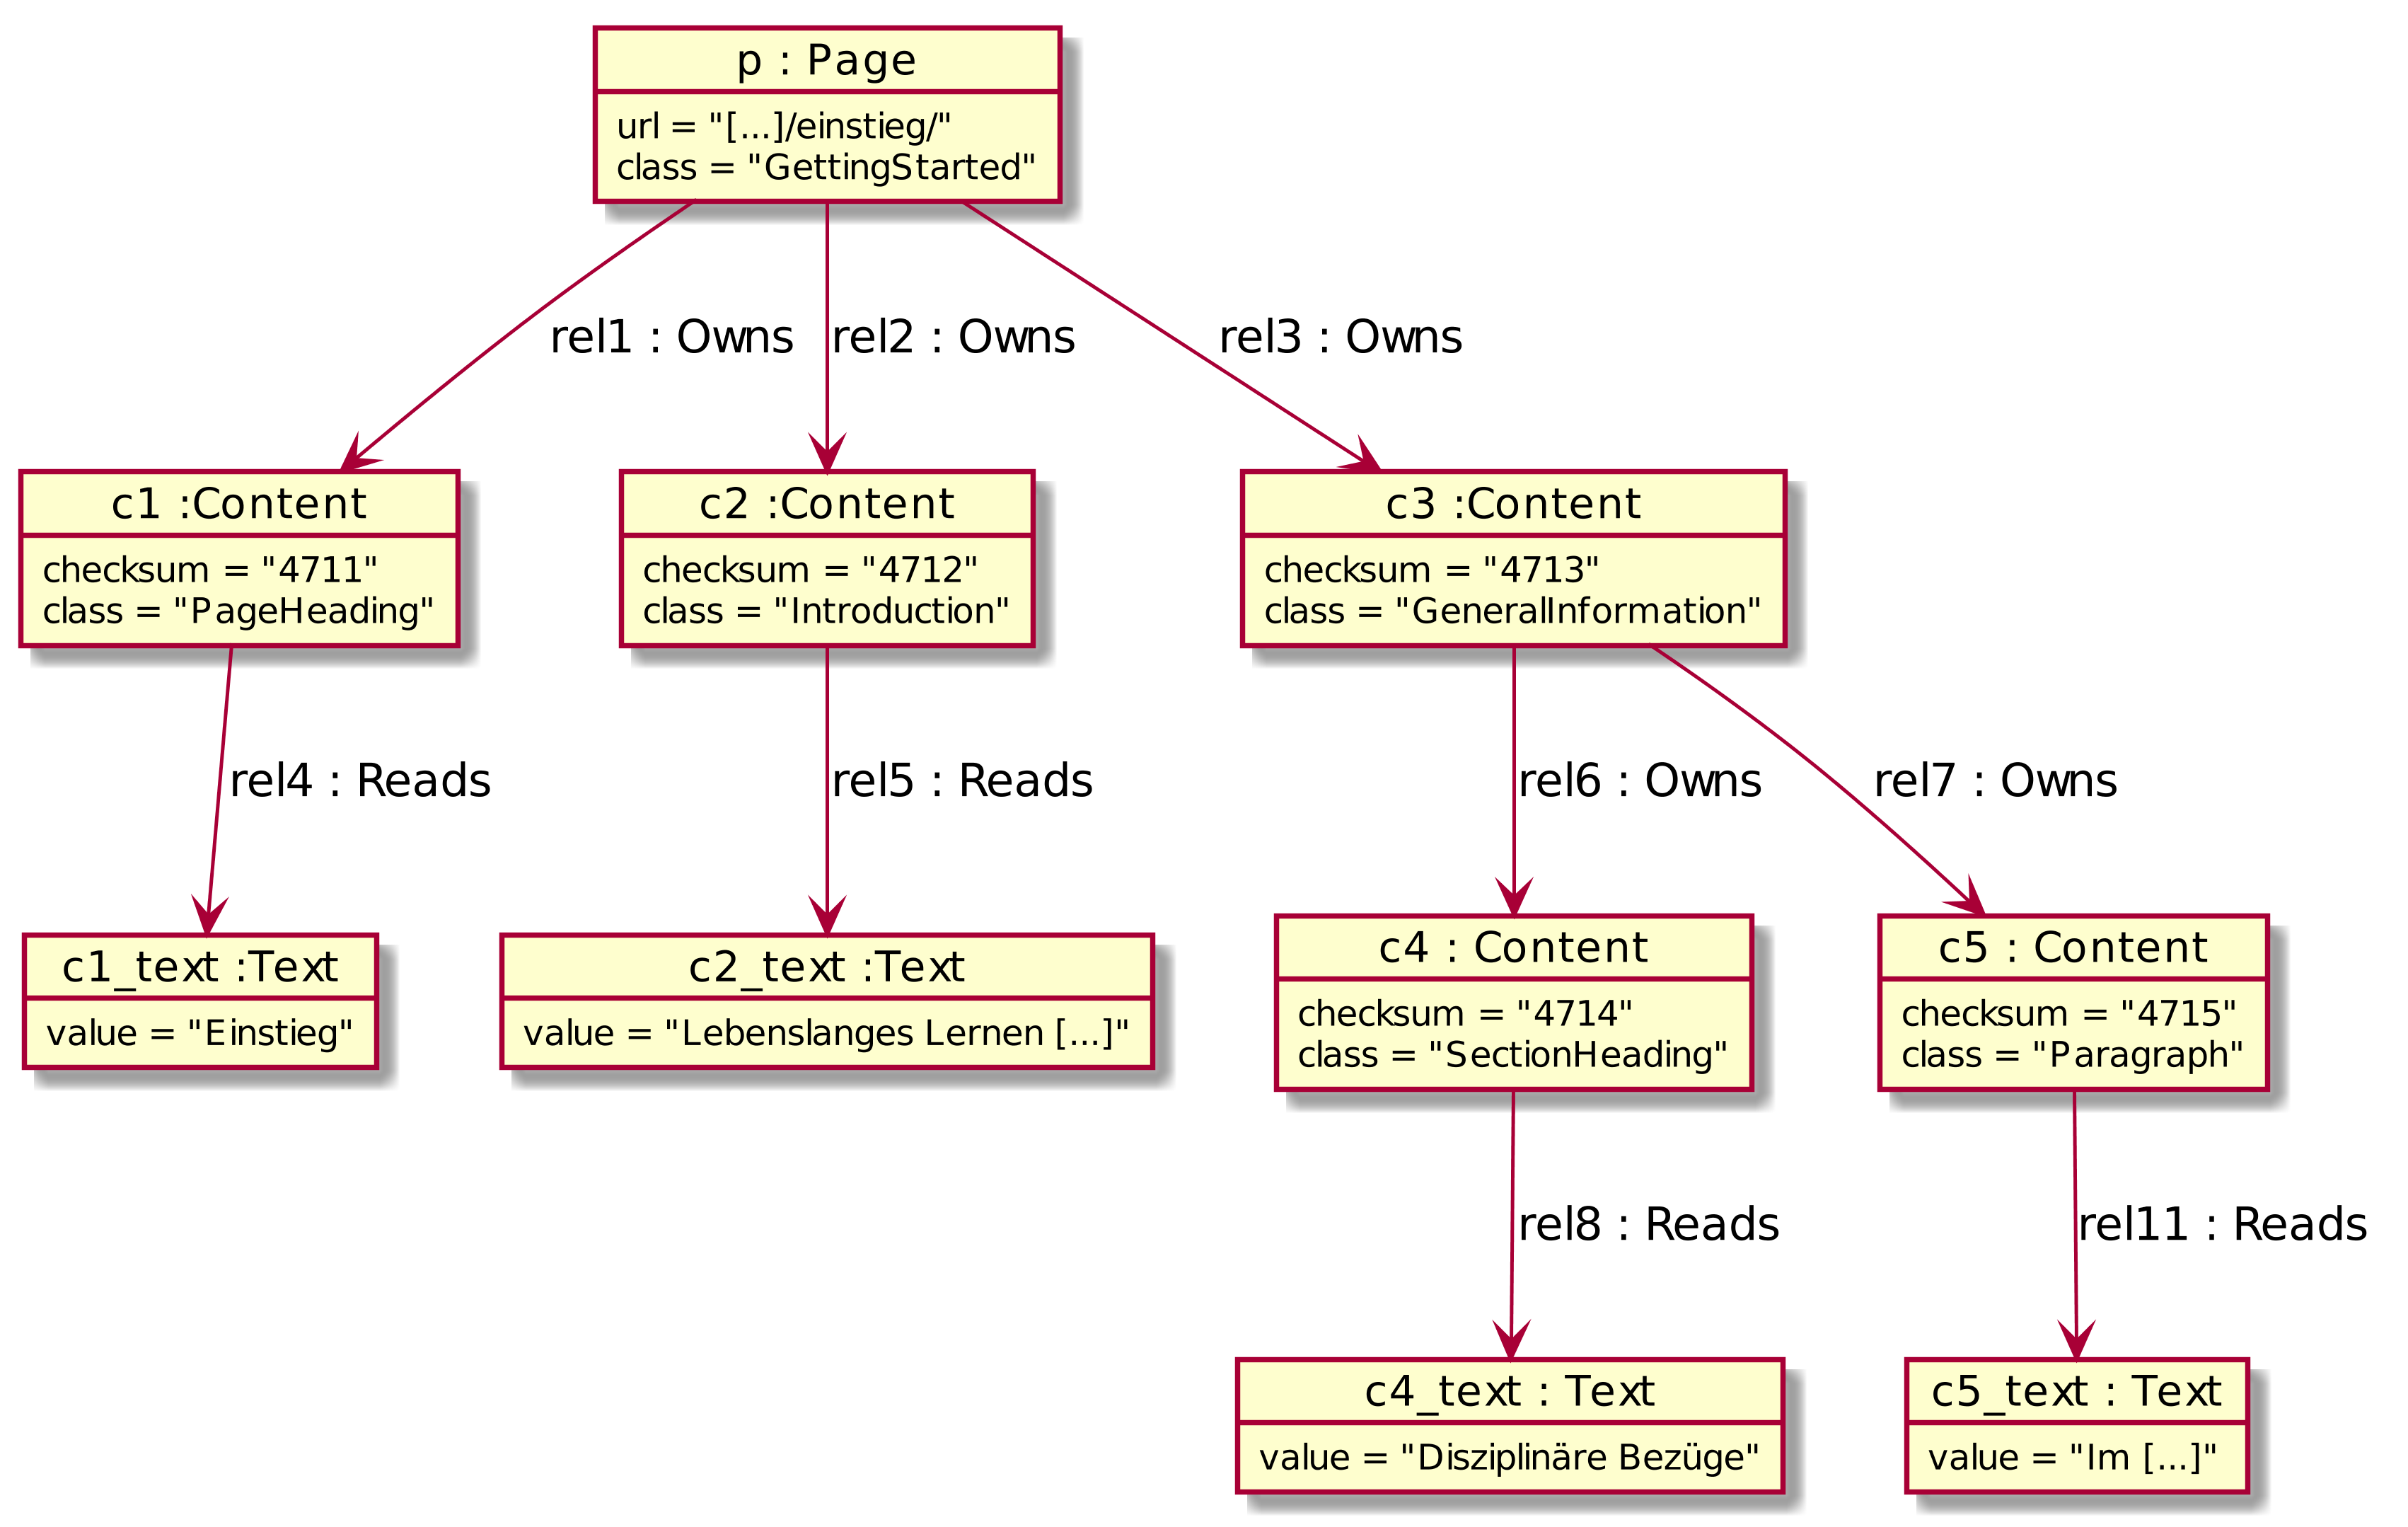
\includegraphics[width=\textwidth]{../resources/db-data-model/example/example_part1.png}
        \caption{Beispiel Teil 1}
        \label{image:dbDataModelExampleOverviewPart1}
    \end{figure}

    Die klassifizierte Seite wurde als "`GettingStarted"' erkannt und besitzt drei skalare Content Features,
    die jeweils durch einen Content Knoten repräsentiert werden und die mit der Seite über
    Owns Beziehungen verknüpft sind.
    Die Contents c1 und c2 beinhalten Text und sind deshalb mit entsprechenden Text Knoten verbunden.
    Hingegen hat c3 zwei eigene Content Features und hat deshalb keinen Text. % TODO Siehe da wo erklärt, dass das doof wäre (oben irgendwo)
    Diese Child Features c4 und c5 besitzen ihrerseits wieder Text.

    Ein weiterer Teil des Beispiels ist zur besseren Übersichtlichkeit in
    Abbildung \ref{image:dbDataModelExampleOverviewPart2} zu sehen.

    \begin{figure}[htb]
        \centering
        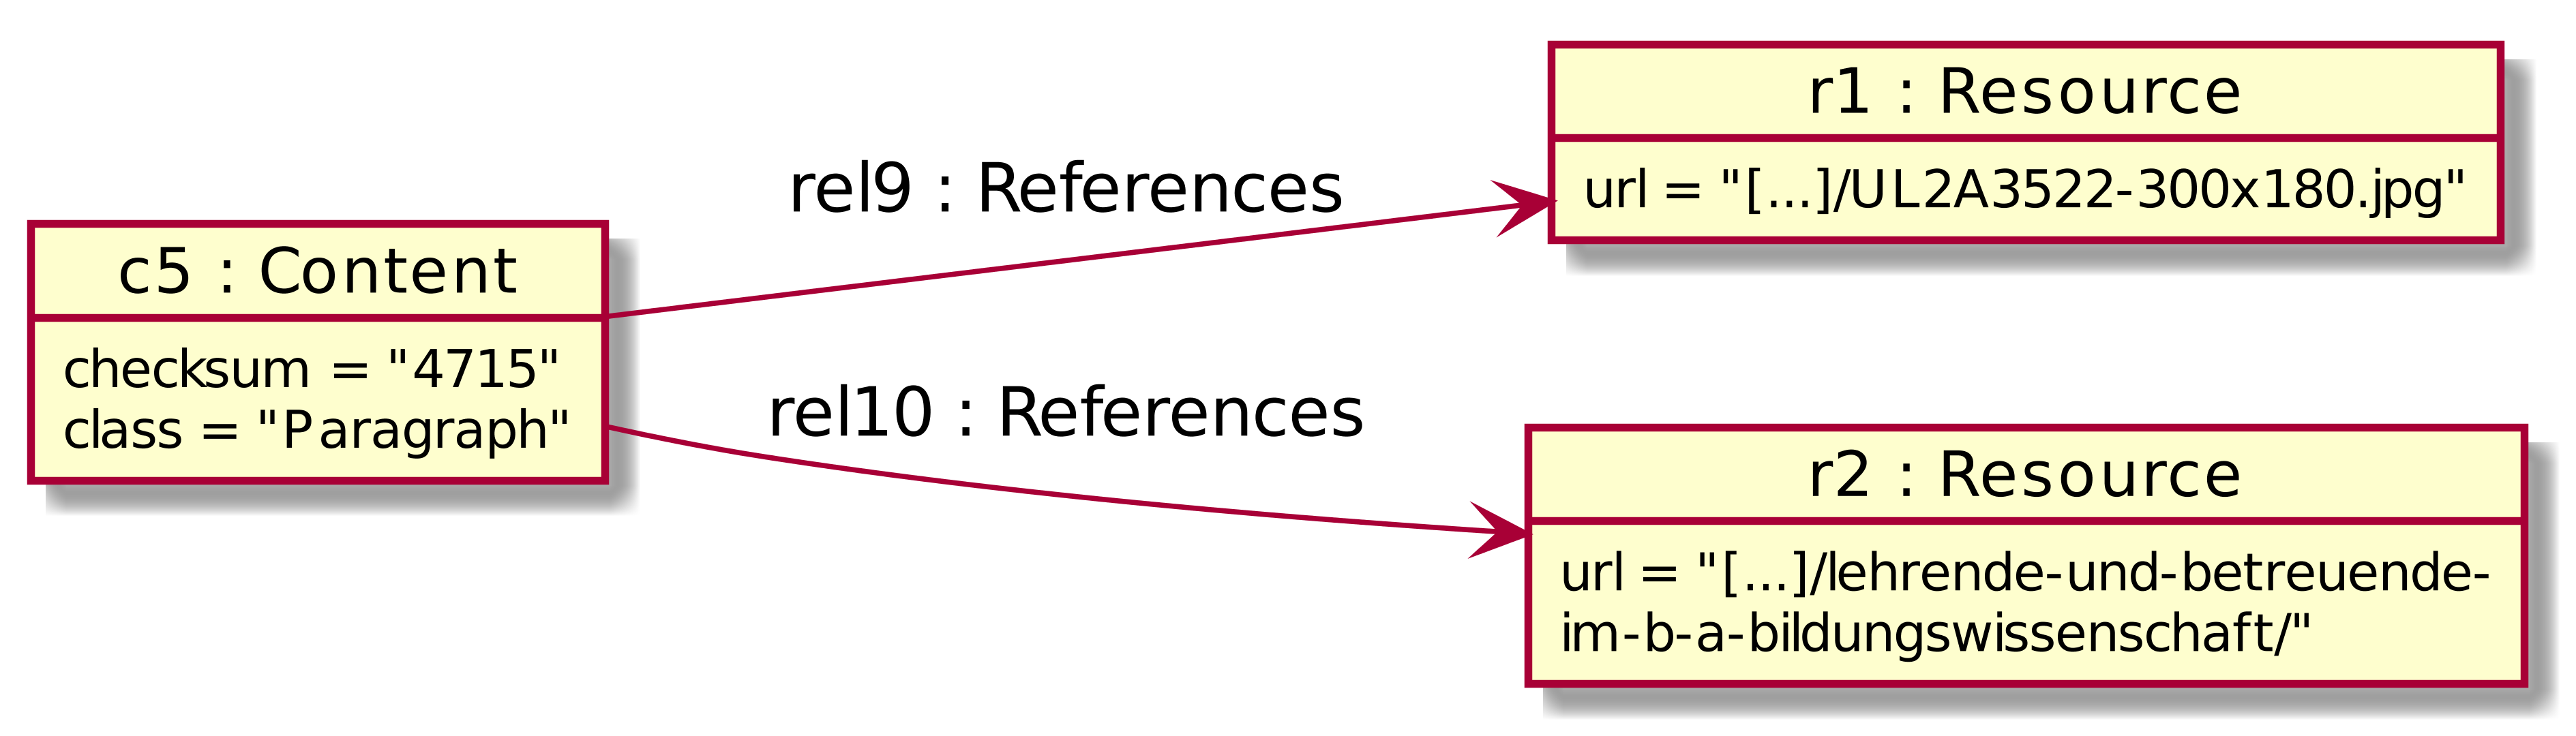
\includegraphics[width=\textwidth]{../resources/db-data-model/example/example_part2.png}
        \caption{Beispiel Teil 2}
        \label{image:dbDataModelExampleOverviewPart2}
    \end{figure}

    Hier ist zu sehen, dass c5 neben seinem Text auch zwei {\resource} referenziert,
    die durch entsprechende Knoten dargestellt werden.
    Bei diesen Referenzen handelt es sich um ein Collection Feature,
    was durch Abbildung \ref{image:dbDataModelExampleRel10} ersichtlich wird.

    \begin{figure}[htb]
        \centering
        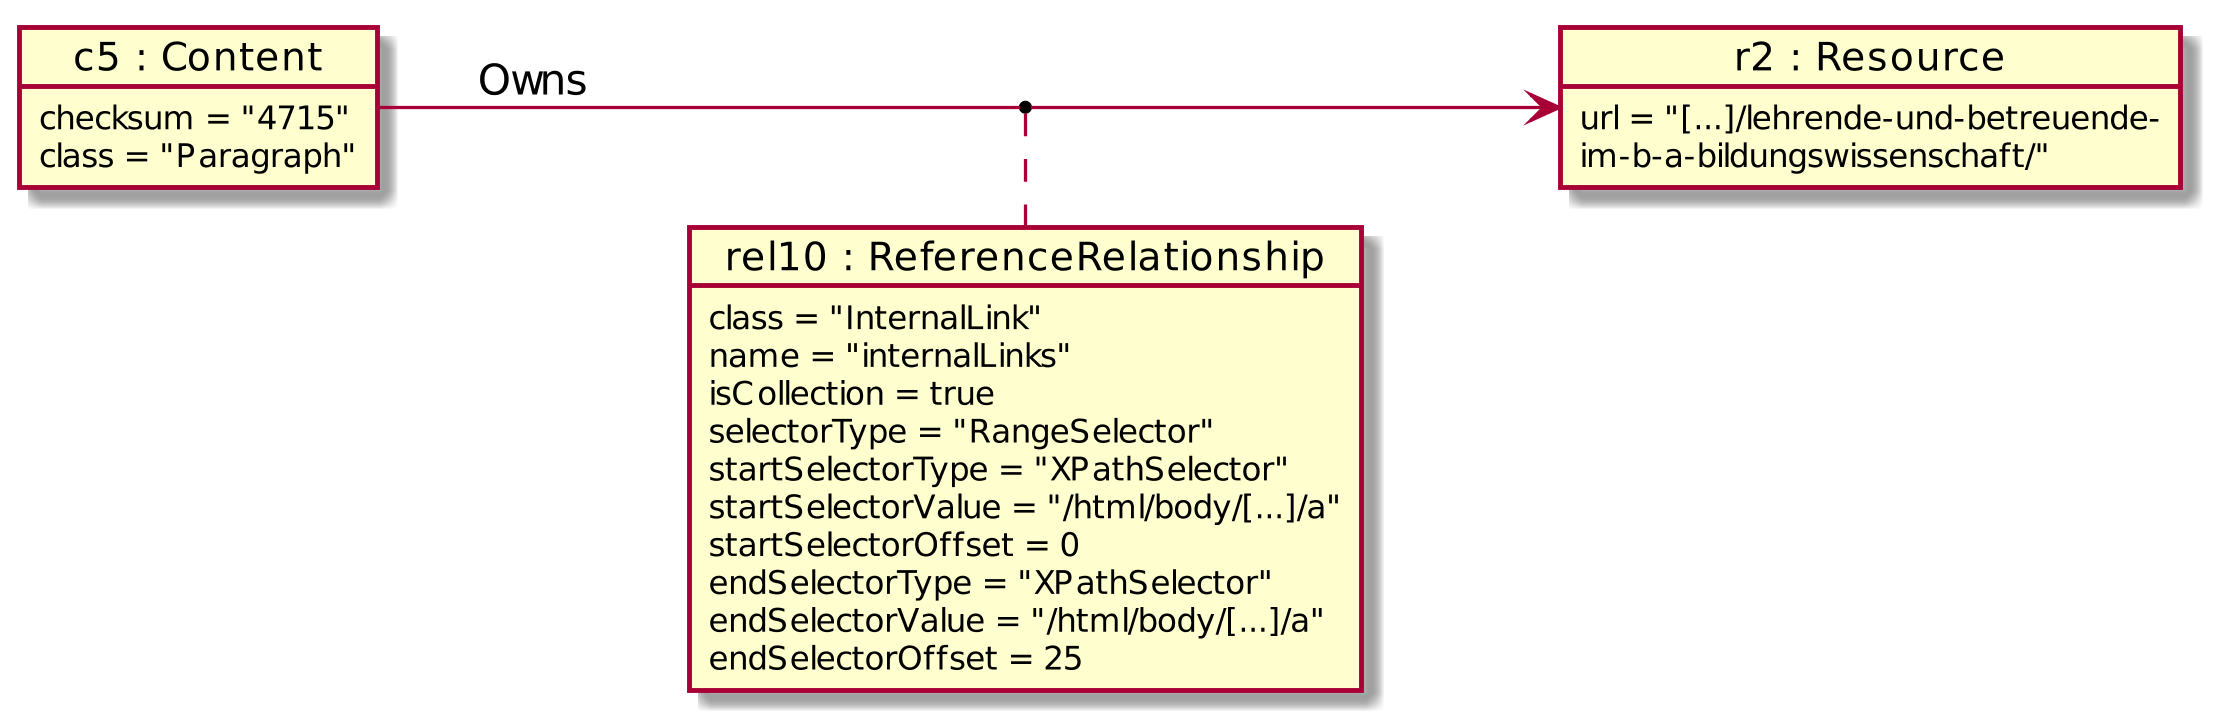
\includegraphics[width=\textwidth]{../resources/db-data-model/example/c5-r2.png}
        \caption{Detailansicht der Beziehung rel10}
        \label{image:dbDataModelExampleRel10}
    \end{figure}

    Neben den konkreten Belegungen der verschiedenen anderen Eigenschaften ist nämlich
    die Eigenschaft isCollection auf true gesetzt.
    Des Weiteren wird hier deutlich, wie die Informationen des eindeutigen Selektors des Nodes gespeichert werden.
    Wie zuvor beschreiben handelt es sich dabei um einen XPath Selektor,
    weshalb start- und endSelectorValue XPath-Ausdrücke enthalten.

    Analog dazu sieht auch eine konkrete Beziehung zu einem Content Feature aus,
    wie aus Abbildung \ref{image:dbDataModelExampleRel1} ersichtlich wird.

    \begin{figure}[htb]
        \centering
        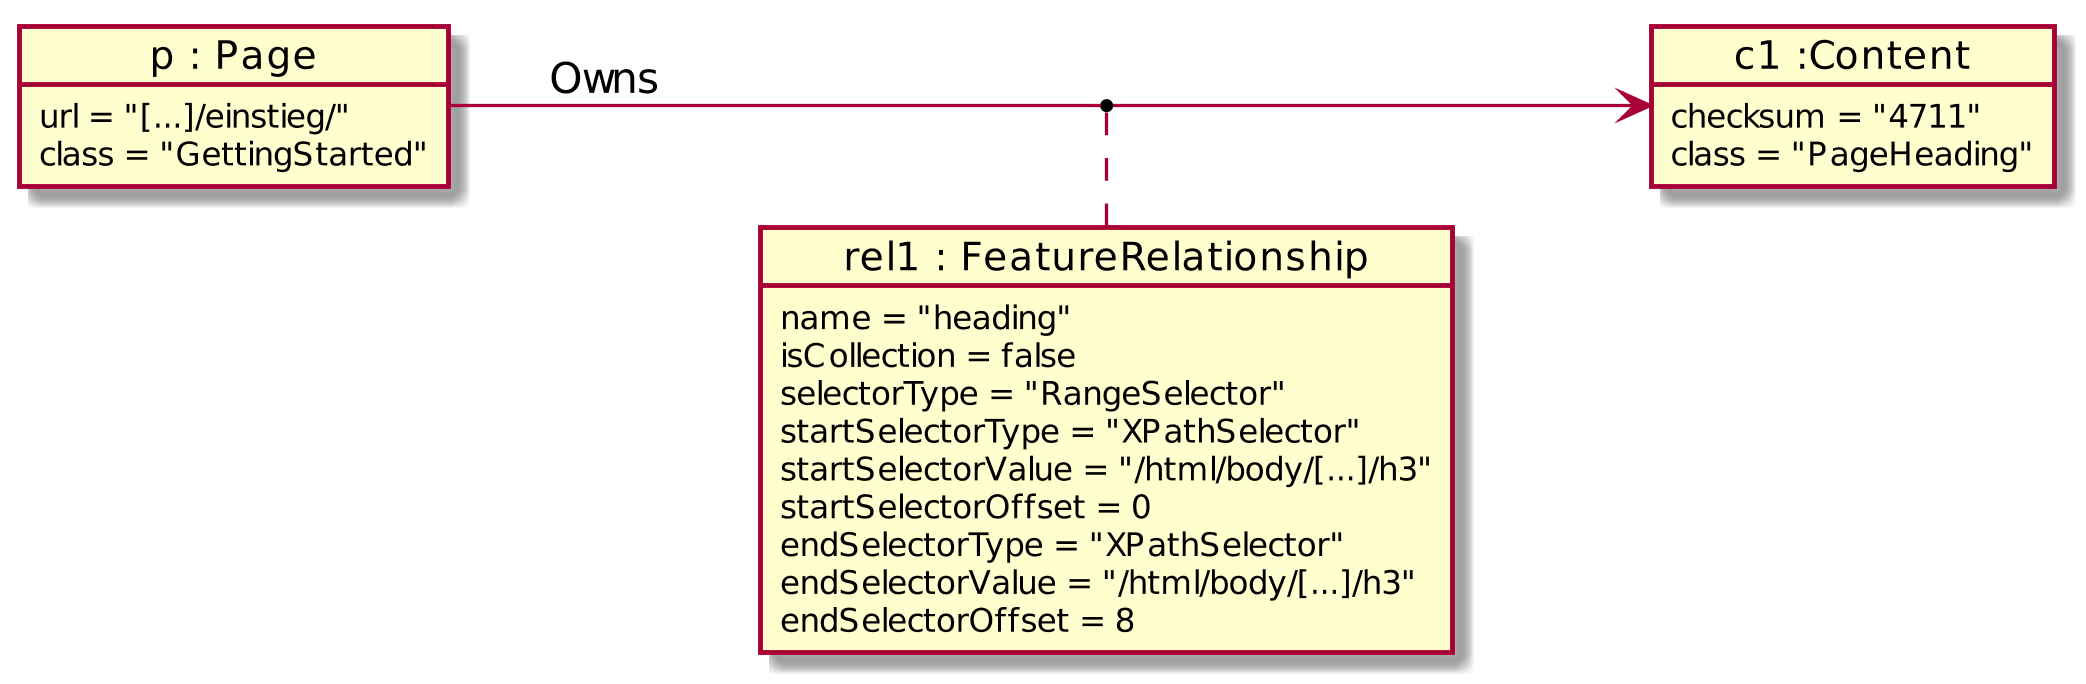
\includegraphics[width=\textwidth]{../resources/db-data-model/example/p-c1.png}
        \caption{Detailansicht der Beziehung rel1}
        \label{image:dbDataModelExampleRel1}
    \end{figure}

    Die Daten folgen dem gleichen Konzept, wie im vorherigen Kapitel beschrieben,
    wird die Klasse allerdings nicht in der Beziehung, sondern im Knoten gespeichert.
